
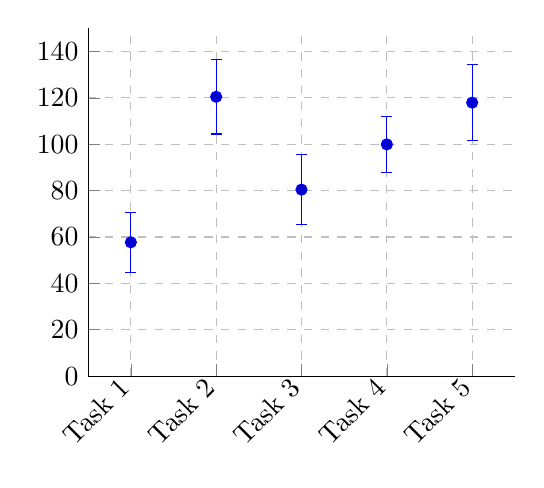
\begin{tikzpicture}[scale=1.0],
\centering
\begin{axis}[
height=6cm,
width=7cm,  
  ymax=150,
  ymin=0,
  xmin=0.5,
  xmax=5.5,
  axis y line*=left,
  axis x line*=bottom,
  xticklabels={Task 1,Task 2,Task 3,Task 4,Task 5},
  xtick={1,...,5},
  ytick={0,20,...,200},
        ymajorgrids=true,
      xmajorgrids=true,
      grid style=dashed,
  x tick label style={rotate=45,anchor=east}]
\addplot+[only marks][error bars/.cd,y dir=both, y explicit]
coordinates {
(1,57.7) +- (12.827,12.827)
(2,120.44) +- (16.041,16.041)
(3,80.409) +- (15.067,15.067)
(4,99.91) +- (11.948,11.948)
(5,117.92) +- (16.31,16.31)
};
\addplot[dashed] coordinates {(0,0) (5.5,0)};
\end{axis}
\end{tikzpicture}%
